
\section{Calculating the \gls{cdf} of arrival time}
\label{sec:etas_cdfs}

The first consideration is that \glspl{eta} are typically displayed as integers, so we need to decide how to round values. For example, 105~seconds is 1.75~minutes: should this be displayed as 2~minutes (standard rounding) or 1~minute (integer rounding)? We will be using Bayesian posterior predictive probabilities, so for example we may want to estimate the median such that $\Pr{A \geq a} = 0.5$; however, if we round $A$ in the above example to 2 minutes, then not only is the equality incorrect, but the probability that the actual arrival time $A$ is after the estimated arrival time $a$ is \emph{less than 0.5}. Therefore, it makes sense to use integer rounding, or the \emph{floor} operator, to find the maximum value of $a \in \{0, 1, 2, \ldots\}$ such that $\Pr{A \geq a} \geq 0.5$.


Computing the \gls{cdf} of arrival time with the particle filter is simple once we have decided on a rounding rule. The arrival time for each particle $\Tarr\vi$ is rounded down, $\lfloor\Tarr\vi\rfloor$, and then tabulated to count how many particles attain each arrival time. Then, the probability that the bus arrives within the interval $[a, a+1), a\in\{0,1,2,\ldots\}$ is given by
\begin{equation}
\label{eq:pf_pdf_arrivaltime}
\Pr{A \in [a, a+1)} =
\frac{\text{number of particles arriving in $a$ to $a+1$~minutes}}{N^\star}
\end{equation}
which leads to the \gls{cdf}
\begin{equation}
\label{eq:pf_cdf_arrivaltime}
\Pr{A < a} = \sum_{x=0}^{x=a-1} \Pr{A \in [x, x+1)}.
\end{equation}
For a chosen stop along a selected trip, this can be graphed, as we have done in \cref{fig:eta_cdf}. The remainder of this chapter explores the choice of summary statistics to display to commuters.

\begin{knitrout}\small
\definecolor{shadecolor}{rgb}{0.969, 0.969, 0.969}\color{fgcolor}\begin{figure}

{\centering 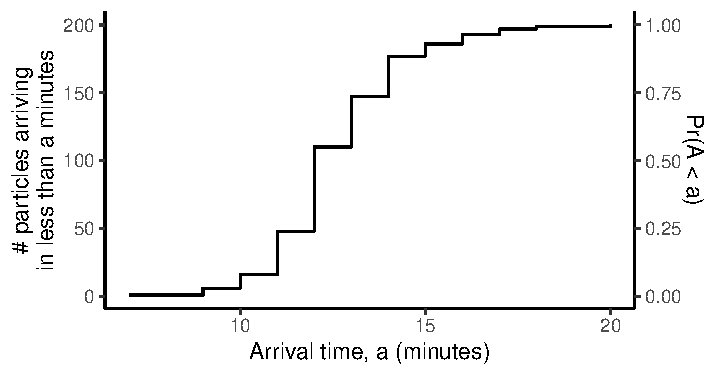
\includegraphics[width=.6\textwidth]{figure/eta_cdf-1} 

}

\caption[CDF of arrival time]{CDF of arrival time.}\label{fig:eta_cdf}
\end{figure}


\end{knitrout}
